% Options for packages loaded elsewhere
% Options for packages loaded elsewhere
\PassOptionsToPackage{unicode}{hyperref}
\PassOptionsToPackage{hyphens}{url}
%
\documentclass[
  9pt,
  ignorenonframetext,
  aspectratio=169,
]{beamer}
\newif\ifbibliography
\usepackage{pgfpages}
\setbeamertemplate{caption}[numbered]
\setbeamertemplate{caption label separator}{: }
\setbeamercolor{caption name}{fg=normal text.fg}
\beamertemplatenavigationsymbolsempty
% remove section numbering
\setbeamertemplate{part page}{
  \centering
  \begin{beamercolorbox}[sep=16pt,center]{part title}
    \usebeamerfont{part title}\insertpart\par
  \end{beamercolorbox}
}
\setbeamertemplate{section page}{
  \centering
  \begin{beamercolorbox}[sep=12pt,center]{section title}
    \usebeamerfont{section title}\insertsection\par
  \end{beamercolorbox}
}
\setbeamertemplate{subsection page}{
  \centering
  \begin{beamercolorbox}[sep=8pt,center]{subsection title}
    \usebeamerfont{subsection title}\insertsubsection\par
  \end{beamercolorbox}
}
% Prevent slide breaks in the middle of a paragraph
\widowpenalties 1 10000
\raggedbottom
\AtBeginPart{
  \frame{\partpage}
}
\AtBeginSection{
  \ifbibliography
  \else
    \frame{\sectionpage}
  \fi
}
\AtBeginSubsection{
  \frame{\subsectionpage}
}
\usepackage{iftex}
\ifPDFTeX
  \usepackage[T1]{fontenc}
  \usepackage[utf8]{inputenc}
  \usepackage{textcomp} % provide euro and other symbols
\else % if luatex or xetex
  \usepackage{unicode-math} % this also loads fontspec
  \defaultfontfeatures{Scale=MatchLowercase}
  \defaultfontfeatures[\rmfamily]{Ligatures=TeX,Scale=1}
\fi
\usepackage{lmodern}

\ifPDFTeX\else
  % xetex/luatex font selection
\fi
% Use upquote if available, for straight quotes in verbatim environments
\IfFileExists{upquote.sty}{\usepackage{upquote}}{}
\IfFileExists{microtype.sty}{% use microtype if available
  \usepackage[]{microtype}
  \UseMicrotypeSet[protrusion]{basicmath} % disable protrusion for tt fonts
}{}
\makeatletter
\@ifundefined{KOMAClassName}{% if non-KOMA class
  \IfFileExists{parskip.sty}{%
    \usepackage{parskip}
  }{% else
    \setlength{\parindent}{0pt}
    \setlength{\parskip}{6pt plus 2pt minus 1pt}}
}{% if KOMA class
  \KOMAoptions{parskip=half}}
\makeatother


\usepackage{longtable,booktabs,array}
\usepackage{calc} % for calculating minipage widths
\usepackage{caption}
% Make caption package work with longtable
\makeatletter
\def\fnum@table{\tablename~\thetable}
\makeatother
\usepackage{graphicx}
\makeatletter
\newsavebox\pandoc@box
\newcommand*\pandocbounded[1]{% scales image to fit in text height/width
  \sbox\pandoc@box{#1}%
  \Gscale@div\@tempa{\textheight}{\dimexpr\ht\pandoc@box+\dp\pandoc@box\relax}%
  \Gscale@div\@tempb{\linewidth}{\wd\pandoc@box}%
  \ifdim\@tempb\p@<\@tempa\p@\let\@tempa\@tempb\fi% select the smaller of both
  \ifdim\@tempa\p@<\p@\scalebox{\@tempa}{\usebox\pandoc@box}%
  \else\usebox{\pandoc@box}%
  \fi%
}
% Set default figure placement to htbp
\def\fps@figure{htbp}
\makeatother





\setlength{\emergencystretch}{3em} % prevent overfull lines

\providecommand{\tightlist}{%
  \setlength{\itemsep}{0pt}\setlength{\parskip}{0pt}}



 


\PassOptionsToPackage{backref=page}{hyperref}
% %%% === ADDITIONAL PACKAGES
% \usepackage{animate}
\usepackage{caption}
\usepackage{subcaption}
\usepackage{tikz}
\usepackage{cancel}
\usepackage{booktabs}
\usepackage{stmaryrd}
\usepackage[export]{adjustbox}
\usepackage{fontawesome5}
\usepackage{algorithmic}
\usepackage{amsmath, amssymb}
\usepackage{yfonts}
\graphicspath{{../files/}}

% % \LinesNumbered
\newcommand{\theHalgorithm}{\arabic{algorithm}}
% \newcommand{\theHtable}{\thetable}
\usepackage[ruled,vlined]{algorithm2e}
\renewcommand{\algorithmicrequire}{\textbf{Input:}}
\renewcommand{\algorithmicensure}{\textbf{Output:}}
\newcommand{\vect}[1]{\boldsymbol{\mathbf{#1}}}

% %%% === CONDITIONAL PACKAGE
\usepackage{ifthen}

%%% === TEMPLATE
\usepackage{fontspec}
\usepackage{polyglossia}

% Set the main language to Russian
% \setmainlanguage{russian}

% Set Computer Modern Unicode (CMU) as the main font for both Latin and Cyrillic
\newfontfamily\cyrillicfont{CMU Serif}
\newfontfamily\cyrillicfontsf{CMU Sans Serif}
\newfontfamily\cyrillicfonttt{CMU Typewriter Text}

\setmainfont{CMU Serif}          % For regular (serif) text
\setsansfont{CMU Sans Serif}      % For sans-serif text
\setmonofont{CMU Typewriter Text} % For monospaced (typewriter-style) text
\DeclareSymbolFontAlphabet{\mathbb}{AMSb}
\setmathfont{CMU Sans Serif}

\setbeamerfont{title}{series=\bfseries}
\setbeamerfont{frametitle}{series=\bfseries, size=\fontsize{12}{14}}
\setbeamerfont{normal text}{series=\mdseries}

\setbeamersize
{
    text margin left=0.214cm,
    text margin right=0.214cm
}

% \usefonttheme[onlymath]{serif}
\setbeamertemplate{bibliography item}{\insertbiblabel}
\setbeamertemplate{itemize items}[circle] % For level-1 itemize
\setbeamertemplate{itemize subitem}[circle] % For level-2 (subitems)
\setbeamertemplate{itemize subsubitem}[circle] % For level-3 (subsubitems)
\captionsetup[figure]{name=Рис.}

\addtobeamertemplate{footline}{\raisebox{-1.3pt}{\href{https://fmin.xyz}{
\includegraphics[height=0.27cm]{logo.pdf}}~} \hspace{0.2cm} \hbox{\insertsection \hspace{0.2cm}} \hfill \href{https://mipt25.fmin.xyz}{\faGem[regular]} \hspace{0.04cm} \href{https://github.com/MerkulovDaniil/mipt25}{\faGithub} \hspace{0.07cm} \href{https://t.me/fminxyz}{\faTelegram} \hspace{0.4cm}\hbox{\insertframenumber \hspace{0.1cm}}
  \vskip0pt
}

\usenavigationsymbolstemplate{}

% %%% === ADDITIONAL COMMANDS
\newcommand*{\Scale}[2][4]{\scalebox{#1}{$#2$}}%
\newcommand{\argmin}{\operatornamewithlimits{argmin}}
\newcommand{\argmax}{\operatornamewithlimits{argmax}}
\newcommand{\la}{\langle}
\newcommand{\ra}{\rangle}

%%% === BACKGROUND IMAGE SETUP
\AtBeginDocument{
  \ifthenelse{\isundefined{\bgimage}}{
    % No background image specified
  }{
    \setbeamertemplate{title page}{
      \begin{tikzpicture}[remember picture,overlay]
        \node[anchor=center, xshift=0pt, yshift=0pt] at (current page.center) {
          \includegraphics[width=1.05\paperwidth, height=1.05\paperheight]{\bgimage}
        };
        \node[fill=white, fill opacity=0.7, text opacity=1, inner sep=10pt, rounded corners=10pt] at (current page.center) {
          \begin{minipage}{0.5\paperwidth}
            \centering
            \usebeamerfont{title}\inserttitle\par
            \vspace*{0.5cm}
            \usebeamerfont{author}\insertauthor\par
            \vspace*{0.5cm}
            \usebeamerfont{institute}\insertinstitute\par
          \end{minipage}
        };
      \end{tikzpicture}
    }
  }
}
\newcommand{\bgimage}{../files/back2.jpeg}
\makeatletter
\@ifpackageloaded{tcolorbox}{}{\usepackage[skins,breakable]{tcolorbox}}
\@ifpackageloaded{fontawesome5}{}{\usepackage{fontawesome5}}
\definecolor{quarto-callout-color}{HTML}{909090}
\definecolor{quarto-callout-note-color}{HTML}{0758E5}
\definecolor{quarto-callout-important-color}{HTML}{CC1914}
\definecolor{quarto-callout-warning-color}{HTML}{EB9113}
\definecolor{quarto-callout-tip-color}{HTML}{00A047}
\definecolor{quarto-callout-caution-color}{HTML}{FC5300}
\definecolor{quarto-callout-color-frame}{HTML}{acacac}
\definecolor{quarto-callout-note-color-frame}{HTML}{4582ec}
\definecolor{quarto-callout-important-color-frame}{HTML}{d9534f}
\definecolor{quarto-callout-warning-color-frame}{HTML}{f0ad4e}
\definecolor{quarto-callout-tip-color-frame}{HTML}{02b875}
\definecolor{quarto-callout-caution-color-frame}{HTML}{fd7e14}
\makeatother
\makeatletter
\@ifpackageloaded{caption}{}{\usepackage{caption}}
\AtBeginDocument{%
\ifdefined\contentsname
  \renewcommand*\contentsname{Table of contents}
\else
  \newcommand\contentsname{Table of contents}
\fi
\ifdefined\listfigurename
  \renewcommand*\listfigurename{List of Figures}
\else
  \newcommand\listfigurename{List of Figures}
\fi
\ifdefined\listtablename
  \renewcommand*\listtablename{List of Tables}
\else
  \newcommand\listtablename{List of Tables}
\fi
\ifdefined\figurename
  \renewcommand*\figurename{Figure}
\else
  \newcommand\figurename{Figure}
\fi
\ifdefined\tablename
  \renewcommand*\tablename{Table}
\else
  \newcommand\tablename{Table}
\fi
}
\@ifpackageloaded{float}{}{\usepackage{float}}
\floatstyle{ruled}
\@ifundefined{c@chapter}{\newfloat{codelisting}{h}{lop}}{\newfloat{codelisting}{h}{lop}[chapter]}
\floatname{codelisting}{Listing}
\newcommand*\listoflistings{\listof{codelisting}{List of Listings}}
\makeatother
\makeatletter
\makeatother
\makeatletter
\@ifpackageloaded{caption}{}{\usepackage{caption}}
\@ifpackageloaded{subcaption}{}{\usepackage{subcaption}}
\makeatother

\usepackage{bookmark}
\IfFileExists{xurl.sty}{\usepackage{xurl}}{} % add URL line breaks if available
\urlstyle{same}
\hypersetup{
  pdftitle={Автоматическое дифференцирование},
  pdfauthor={Даниил Меркулов},
  hidelinks,
  pdfcreator={LaTeX via pandoc}}


\title{Автоматическое дифференцирование}
\author{Даниил Меркулов}
\date{}
\institute{Методы оптимизации. МФТИ}

\begin{document}
\frame{\titlepage}


\section{Повторим матричное
дифференцирование}\label{ux43fux43eux432ux442ux43eux440ux438ux43c-ux43cux430ux442ux440ux438ux447ux43dux43eux435-ux434ux438ux444ux444ux435ux440ux435ux43dux446ux438ux440ux43eux432ux430ux43dux438ux435}

\begin{frame}{Пример 1}
\phantomsection\label{ux43fux440ux438ux43cux435ux440-1}
\begin{tcolorbox}[enhanced jigsaw, bottomrule=.15mm, title=\textcolor{quarto-callout-color}{\faInfo}\hspace{0.5em}{Example}, breakable, opacitybacktitle=0.6, colbacktitle=quarto-callout-color!10!white, left=2mm, bottomtitle=1mm, colback=white, colframe=quarto-callout-color-frame, titlerule=0mm, toptitle=1mm, arc=.35mm, rightrule=.15mm, coltitle=black, toprule=.15mm, opacityback=0, leftrule=.75mm]

Найти гессиан \(\nabla^2 f(x)\), если
\(f(x) = \langle x, Ax\rangle -b^T x + c\).

\end{tcolorbox}

\pause

\begin{columns}[T]
\begin{column}{0.5\linewidth}
\begin{enumerate}[<+->]
\item
  Распишем дифференциал \(df\) \[
   \begin{split}
   df &= d\left(\langle Ax, x\rangle - \langle b, x\rangle + c\right) \\
   &= \langle Ax, dx\rangle + \langle x, Adx\rangle - \langle b, dx\rangle \\
   &= \langle Ax, dx\rangle + \langle A^Tx, dx\rangle - \langle b, dx\rangle \\
   &= \langle (A+A^T)x - b, dx\rangle  \\
   \end{split}
   \]

  Что означает, что градиент \(\nabla f = (A+A^T)x - b\).
\end{enumerate}
\end{column}

\pause

\begin{column}{0.5\linewidth}
\begin{enumerate}[<+->]
\setcounter{enumi}{1}
\item
  Найдем второй дифференциал \(d^2f = d(df)\), полагая, что
  \(dx=dx_1 = \text{const}\): \[
   \begin{split}
   d^2f &= d\left(\langle (A+A^T)x - b, dx_1\rangle\right) \\
   &= \langle (A+A^T)dx, dx_1\rangle \\
   &= \langle dx, (A+A^T)^Tdx_1\rangle \\
   &= \langle (A+A^T)dx_1, dx\rangle 
   \end{split}
   \]

  Таким образом, гессиан: \(\nabla^2 f = (A+A^T)\).
\end{enumerate}
\end{column}
\end{columns}
\end{frame}

\begin{frame}{Пример 2}
\phantomsection\label{ux43fux440ux438ux43cux435ux440-2}
\begin{tcolorbox}[enhanced jigsaw, bottomrule=.15mm, title=\textcolor{quarto-callout-color}{\faInfo}\hspace{0.5em}{Example}, breakable, opacitybacktitle=0.6, colbacktitle=quarto-callout-color!10!white, left=2mm, bottomtitle=1mm, colback=white, colframe=quarto-callout-color-frame, titlerule=0mm, toptitle=1mm, arc=.35mm, rightrule=.15mm, coltitle=black, toprule=.15mm, opacityback=0, leftrule=.75mm]

Найти гессиан \(\nabla^2 f(x)\), если
\(f(x) = \ln \langle x, Ax\rangle\).

\end{tcolorbox}
\end{frame}

\begin{frame}{Пример 3}
\phantomsection\label{ux43fux440ux438ux43cux435ux440-3}
\begin{tcolorbox}[enhanced jigsaw, bottomrule=.15mm, title=\textcolor{quarto-callout-color}{\faInfo}\hspace{0.5em}{Example}, breakable, opacitybacktitle=0.6, colbacktitle=quarto-callout-color!10!white, left=2mm, bottomtitle=1mm, colback=white, colframe=quarto-callout-color-frame, titlerule=0mm, toptitle=1mm, arc=.35mm, rightrule=.15mm, coltitle=black, toprule=.15mm, opacityback=0, leftrule=.75mm]

Найти градиент \(\nabla f(x)\) и гессиан \(\nabla^2f(x)\), если
\(f(x) = \ln \left( 1 + \exp\langle a,x\rangle\right)\)

\end{tcolorbox}

\pause

\begin{columns}[T]
\begin{column}{0.5\linewidth}
\begin{enumerate}[<+->]
\item
  Начнем с записи дифференциала \(df\). Имеем: \[
   f(x) = \ln \left( 1 + \exp\langle a, x\rangle\right)
   \]

  Используя правило дифференцирования сложной функции: \[
   df = d \left( \ln \left( 1 + \exp\langle a, x\rangle\right) \right)
   = \frac{d \left( 1 + \exp\langle a, x\rangle \right)}{1 + \exp\langle a, x\rangle}
   \]

  теперь посчитаем дифференциал экспоненты: \[
   d \left( \exp\langle a, x\rangle \right) = \exp\langle a, x\rangle \langle a, dx\rangle
   \]

  Подставляя в выражение выше, имеем: \[
   df = \frac{\exp\langle a, x\rangle \langle a, dx\rangle}{1 + \exp\langle a, x\rangle}
   \]
\end{enumerate}
\end{column}

\pause

\begin{column}{0.5\linewidth}
\begin{enumerate}[<+->]
\setcounter{enumi}{1}
\item
  Для выражения \(df\) в нужной форме, запишем: \[
   df = \left\langle \frac{\exp\langle a, x\rangle}{1 + \exp\langle a, x\rangle} a, dx\right\rangle
   \]

  Напомним, что функция сигмоиды определяется как: \[
   \sigma(t) = \frac{1}{1 + \exp(-t)}
   \] Таким образом, мы можем переписать дифференциал: \[
   df = \langle \sigma(\langle a, x\rangle) a, dx \rangle
   \]

  Следовательно, градиент: \[
   \nabla f(x) = \sigma(\langle a, x\rangle) a
   \]
\end{enumerate}
\end{column}
\end{columns}
\end{frame}

\begin{frame}[noframenumbering]{Пример 3}
\phantomsection\label{ux43fux440ux438ux43cux435ux440-3-1}
\begin{tcolorbox}[enhanced jigsaw, bottomrule=.15mm, title=\textcolor{quarto-callout-color}{\faInfo}\hspace{0.5em}{Example}, breakable, opacitybacktitle=0.6, colbacktitle=quarto-callout-color!10!white, left=2mm, bottomtitle=1mm, colback=white, colframe=quarto-callout-color-frame, titlerule=0mm, toptitle=1mm, arc=.35mm, rightrule=.15mm, coltitle=black, toprule=.15mm, opacityback=0, leftrule=.75mm]

Найти градиент \(\nabla f(x)\) и гессиан \(\nabla^2f(x)\), если
\(f(x) = \ln \left( 1 + \exp\langle a,x\rangle\right)\)

\end{tcolorbox}

\begin{enumerate}[<+->]
\setcounter{enumi}{2}
\item
  Теперь найдем гессиан с помозью второго дифференциала: \[
   d(\nabla f(x)) = d\left( \sigma(\langle a, x\rangle) a \right)
   \] Так как вектор \(a\) константа, нам необходимо продифференцировать
  лишь сигмоиду: \[
   d\left( \sigma(\langle a, x\rangle) \right) = \sigma(\langle a, x\rangle)(1 - \sigma(\langle a, x\rangle)) \langle a, dx\rangle
   \]

  То есть: \[
   d(\nabla f(x)) = \sigma(\langle a, x\rangle)(1 - \sigma(\langle a, x\rangle)) \langle a, dx\rangle a
   \]

  Запишем гессиан: \[
   \nabla^2 f(x) = \sigma(\langle a, x\rangle)(1 - \sigma(\langle a, x\rangle)) a a^T
   \]
\end{enumerate}
\end{frame}

\section{Автоматическое
дифференцирование}\label{ux430ux432ux442ux43eux43cux430ux442ux438ux447ux435ux441ux43aux43eux435-ux434ux438ux444ux444ux435ux440ux435ux43dux446ux438ux440ux43eux432ux430ux43dux438ux435}

\begin{frame}[plain]{}
\phantomsection\label{section}
\begin{figure}[H]

{\centering \pandocbounded{
\includegraphics[keepaspectratio]{autograd_expectations.jpeg}}

}

\caption{Когда понял идею}

\end{figure}%
\end{frame}

\begin{frame}[plain]{}
\phantomsection\label{section-1}
\begin{figure}[H]

{\centering 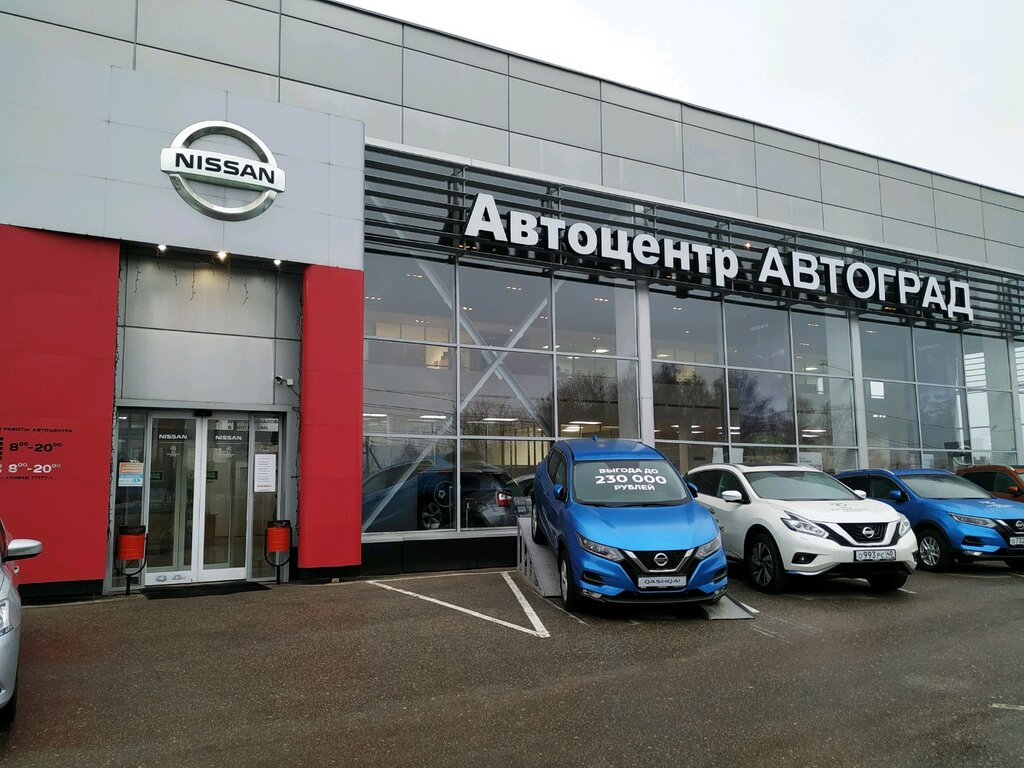
\includegraphics[width=0.65\linewidth,height=\textheight,keepaspectratio]{avtograd.jpeg}

}

\caption{Это не автоград}

\end{figure}%
\end{frame}

\begin{frame}{Задача}
\phantomsection\label{ux437ux430ux434ux430ux447ux430}
Пусть есть задача оптимизации:

\[
L(w) \to \min_{w \in \mathbb{R}^d}
\]

\pause

\begin{itemize}[<+->]
\tightlist
\item
  Such problems typically arise in machine learning, when you need to
  find optimal hyperparameters \(w\) of an ML model (i.e.~train a neural
  network).
\item
  You may use a lot of algorithms to approach this problem, but given
  the modern size of the problem, where \(d\) could be dozens of
  billions it is very challenging to solve this problem without
  information about the gradients using zero-order optimization
  algorithms.
\item
  That is why it would be beneficial to be able to calculate the
  gradient vector
  \(\nabla_w L = \left( \frac{\partial L}{\partial w_1}, \ldots, \frac{\partial L}{\partial w_d}\right)^T\).
\item
  Typically, first-order methods perform much better in huge-scale
  optimization, while second-order methods require too much memory.
\end{itemize}
\end{frame}

\begin{frame}{Пример: задача многомерного шкалирования}
\phantomsection\label{ux43fux440ux438ux43cux435ux440-ux437ux430ux434ux430ux447ux430-ux43cux43dux43eux433ux43eux43cux435ux440ux43dux43eux433ux43e-ux448ux43aux430ux43bux438ux440ux43eux432ux430ux43dux438ux44f}
Suppose, we have a pairwise distance matrix for \(N\) \(d\)-dimensional
objects \(D \in \mathbb{R}^{N \times N}\). Given this matrix, our goal
is to recover the initial coordinates
\(W_i \in \mathbb{R}^d, \; i = 1, \ldots, N\).

\pause

\[
L(W) = \sum_{i, j = 1}^N \left(\|W_i - W_j\|^2_2 - D_{i,j}\right)^2 \to \min_{W \in \mathbb{R}^{N \times d}}
\]

\pause

Link to a nice visualization
\href{http://www.benfrederickson.com/numerical-optimization/}{\(\clubsuit\)},
where one can see, that gradient-free methods handle this problem much
slower, especially in higher dimensions.

\begin{tcolorbox}[enhanced jigsaw, bottomrule=.15mm, title=\textcolor{quarto-callout-color}{\faInfo}\hspace{0.5em}{Question}, breakable, opacitybacktitle=0.6, colbacktitle=quarto-callout-color!10!white, left=2mm, bottomtitle=1mm, colback=white, colframe=quarto-callout-color-frame, titlerule=0mm, toptitle=1mm, arc=.35mm, rightrule=.15mm, coltitle=black, toprule=.15mm, opacityback=0, leftrule=.75mm]

Is it somehow connected with PCA?

\end{tcolorbox}
\end{frame}

\begin{frame}{Пример: задача многомерного шкалирования}
\phantomsection\label{ux43fux440ux438ux43cux435ux440-ux437ux430ux434ux430ux447ux430-ux43cux43dux43eux433ux43eux43cux435ux440ux43dux43eux433ux43e-ux448ux43aux430ux43bux438ux440ux43eux432ux430ux43dux438ux44f-1}
\begin{figure}[H]

{\centering 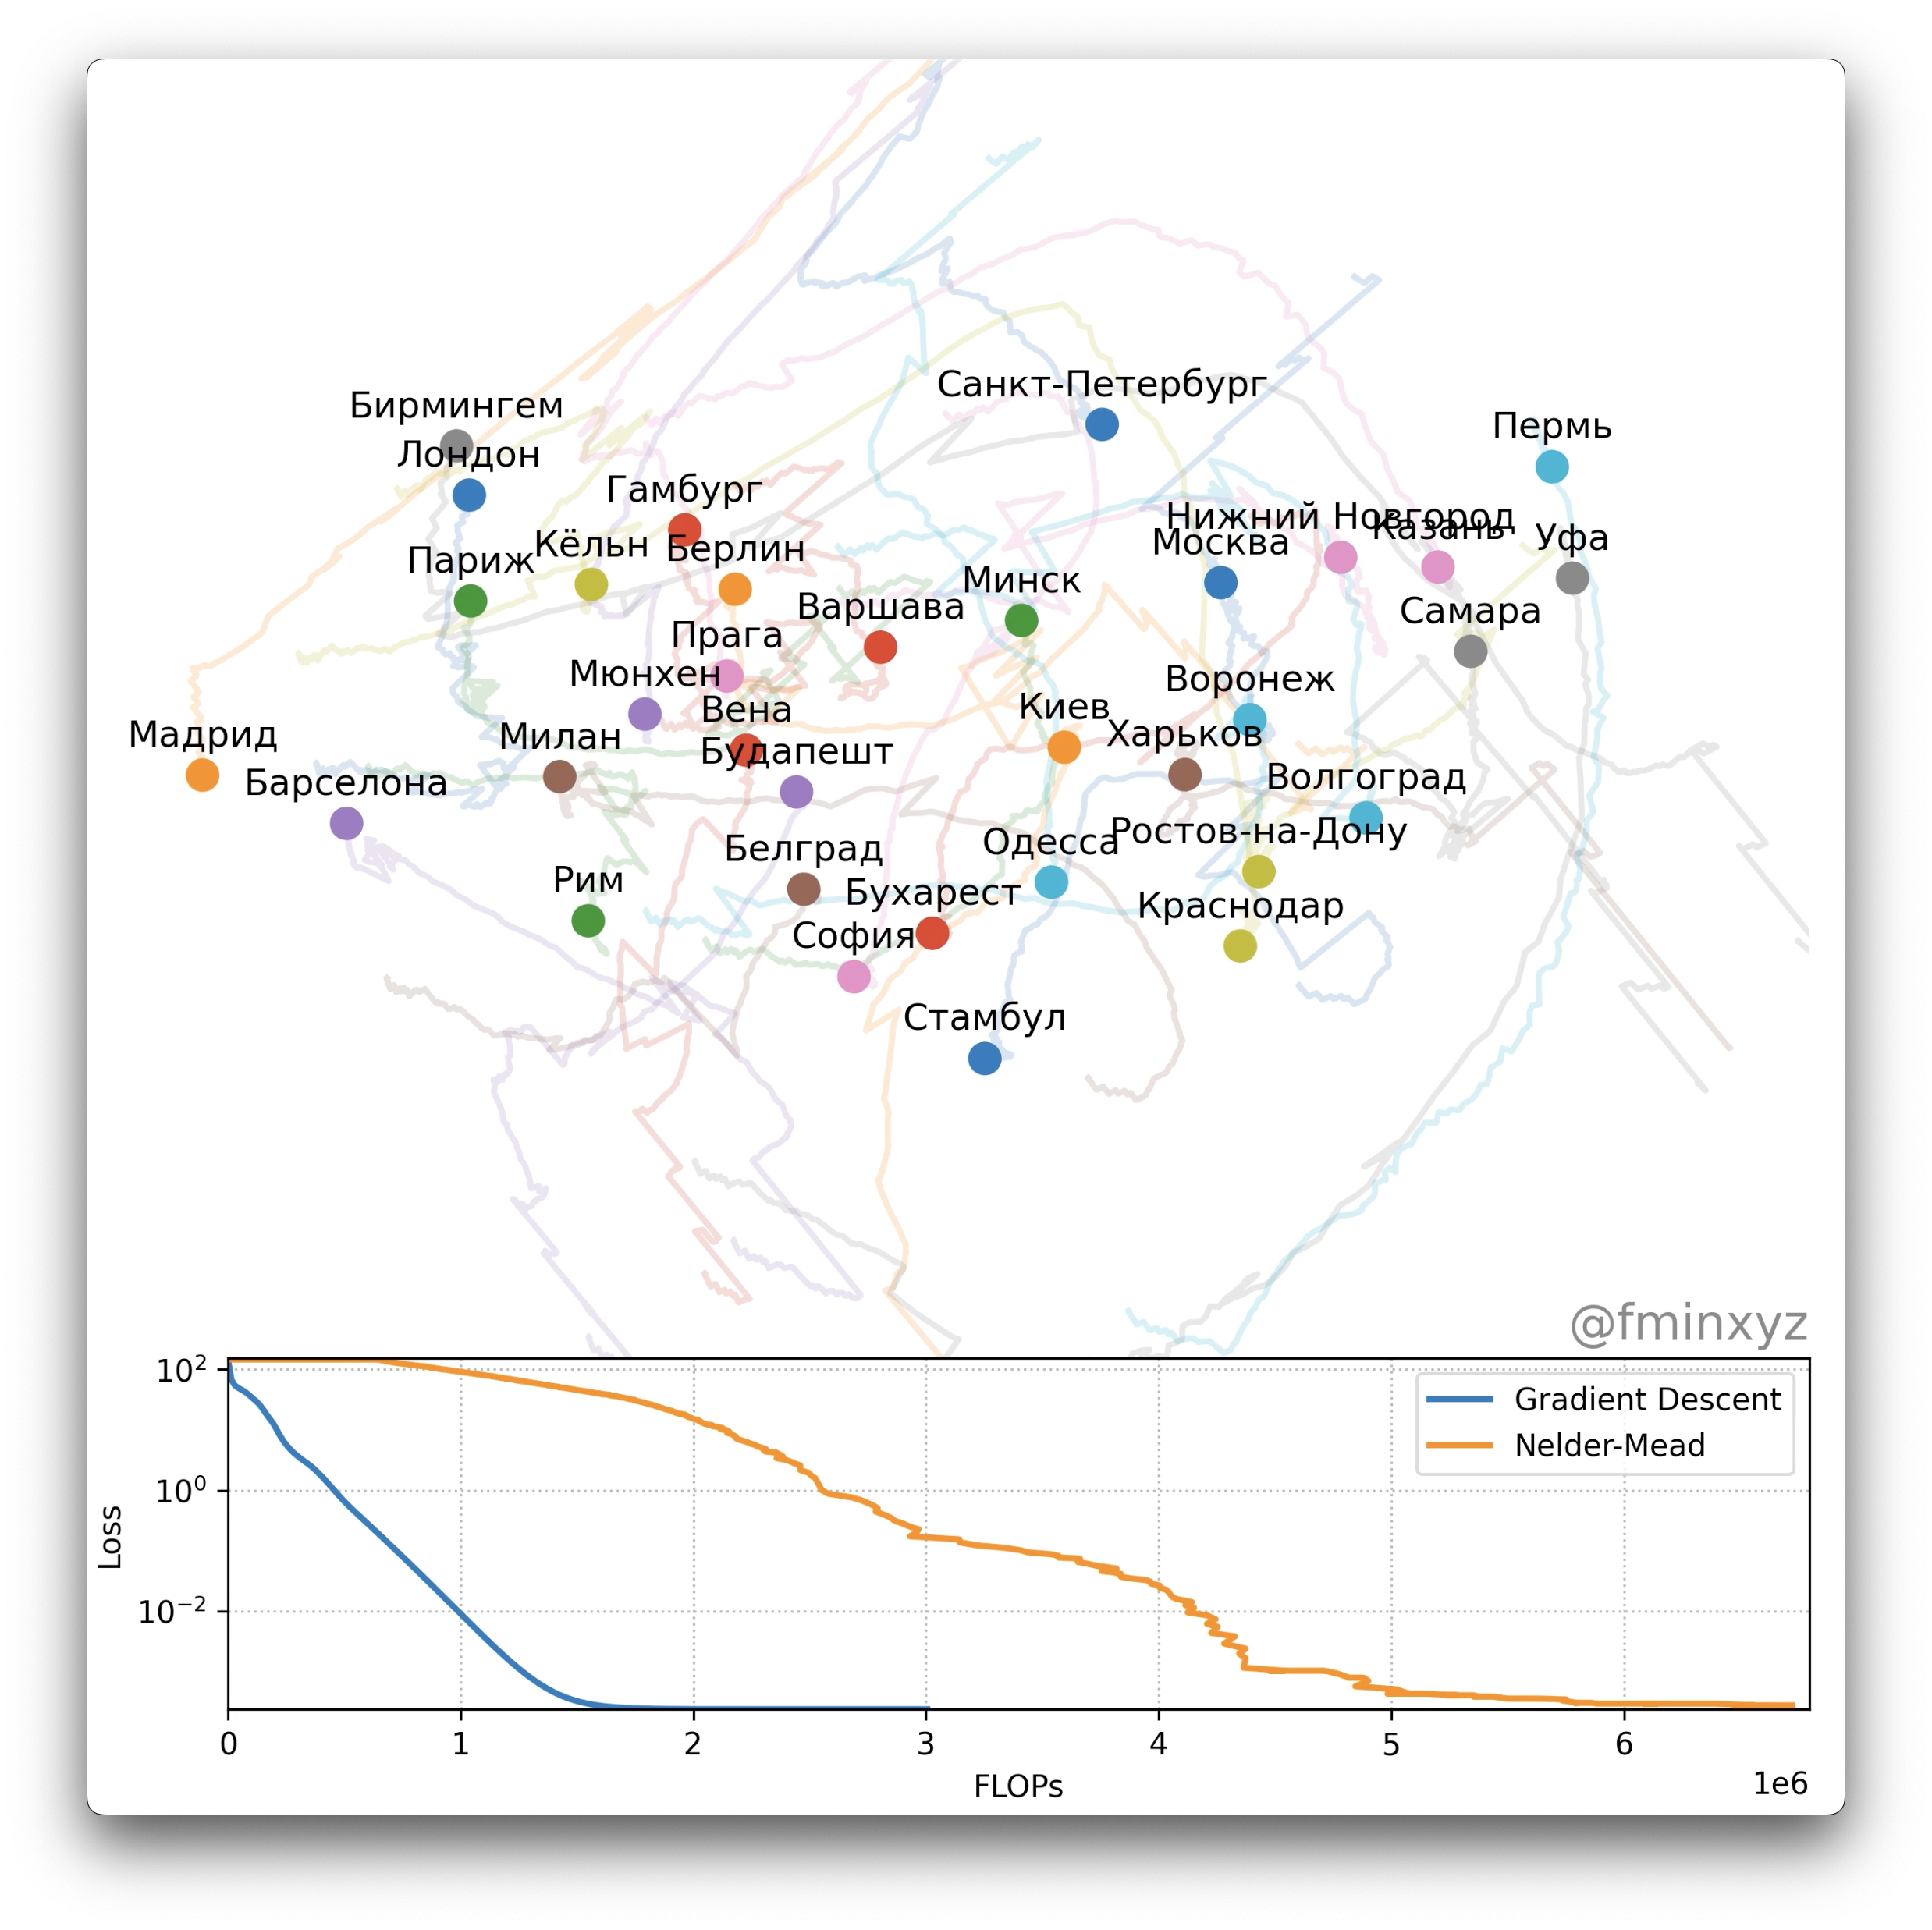
\includegraphics[width=0.4\linewidth,height=\textheight,keepaspectratio]{mds.png}

}

\caption{\href{https://getfile.dokpub.com/yandex/get/https://disk.yandex.ru/i/B5uvsro-y6UCkw}{Ссылка
на анимацию}}

\end{figure}%
\end{frame}

\begin{frame}{Пример: безградиентный градиентный спуск}
\phantomsection\label{ux43fux440ux438ux43cux435ux440-ux431ux435ux437ux433ux440ux430ux434ux438ux435ux43dux442ux43dux44bux439-ux433ux440ux430ux434ux438ux435ux43dux442ux43dux44bux439-ux441ux43fux443ux441ux43a}
\begin{columns}[T]
\begin{column}{0.5\linewidth}
Рассмотрим следующую задачу оптимизации

\[
L(w) \to \min_{w \in \mathbb{R}^d}
\]

\pause

вместе с методом градиентного спуска (GD)

\[
w_{k+1} = w_k - \alpha_k \nabla_w L(w_k)
\]

\pause

Можно ли заменить \(\nabla_w L(w_k)\), используя, лишь информацию
нулевого порядка о функции?

\pause

Да, но есть нюанс.

\pause

One can consider 2-point gradient estimator\footnote<.->[frame]{I
  suggest a
  \href{https://scholar.harvard.edu/files/yujietang/files/slides_2019_zero-order_opt_tutorial.pdf}{nice}
  presentation about gradient-free methods} \(G\):

\[
G = d\dfrac{L(w + \varepsilon v)- L(w - \varepsilon v)}{2 \varepsilon}v, 
\]

where \(v\) is spherically symmetric.
\end{column}

\pause

\begin{column}{0.5\linewidth}
\begin{figure}[H]

{\centering \pandocbounded{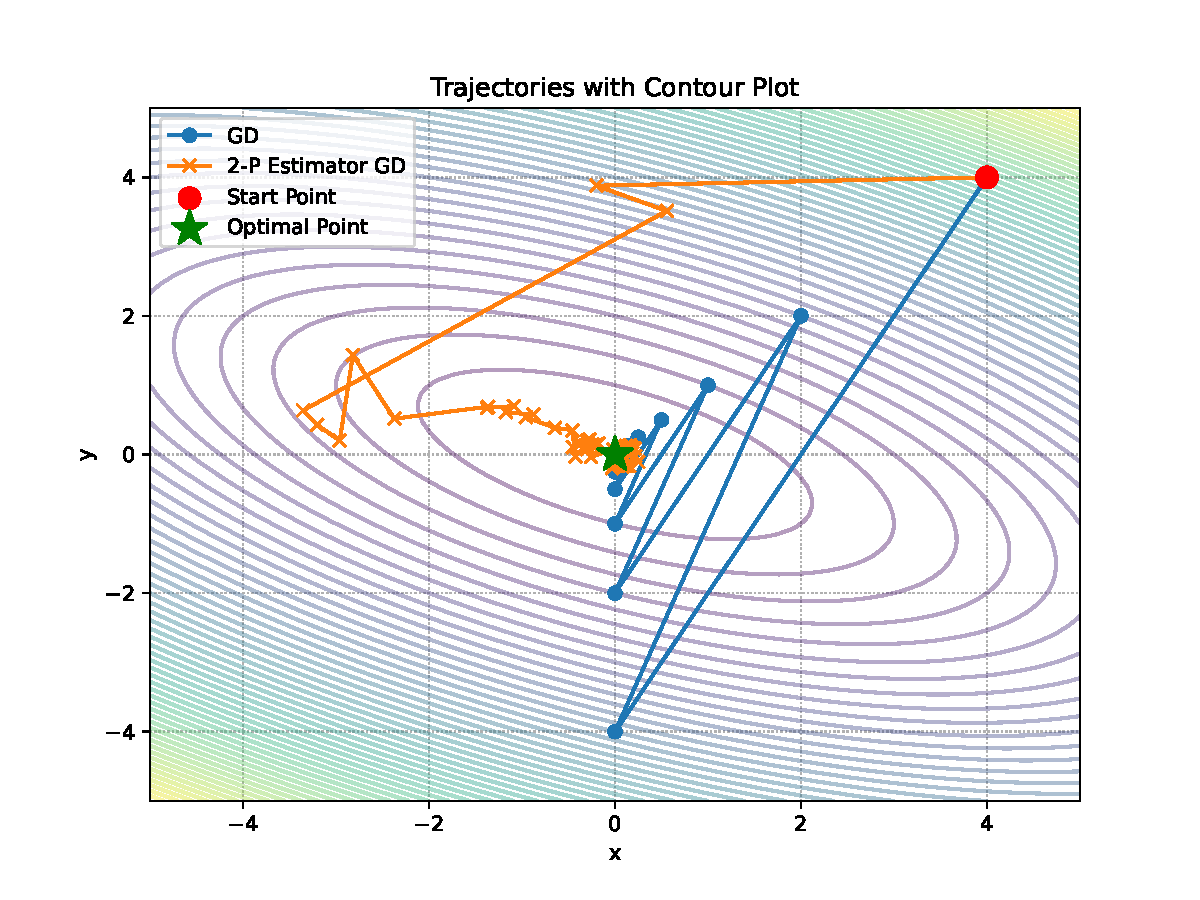
\includegraphics[keepaspectratio]{zgd_2p.pdf}}

}

\caption{``Illustration of two-point estimator of Gradient Descent''}

\end{figure}%
\end{column}
\end{columns}
\end{frame}

\begin{frame}{Пример: конечно-разностный градиентный спуск}
\phantomsection\label{ux43fux440ux438ux43cux435ux440-ux43aux43eux43dux435ux447ux43dux43e-ux440ux430ux437ux43dux43eux441ux442ux43dux44bux439-ux433ux440ux430ux434ux438ux435ux43dux442ux43dux44bux439-ux441ux43fux443ux441ux43a}
\begin{columns}[T]
\begin{column}{0.5\linewidth}
\[
w_{k+1} = w_k - \alpha_k G
\]

\pause

One can also consider the idea of finite differences:

\[
G =  \sum\limits_{i=1}^d\dfrac{L(w+\varepsilon e_i) - L(w-\varepsilon e_i)}{2\varepsilon} e_i
\]

\href{https://colab.research.google.com/github/MerkulovDaniil/optim/blob/master/assets/Notebooks/Zero_order_GD.ipynb}{Open
In Colab \(\clubsuit\)}
\end{column}

\begin{column}{0.5\linewidth}
\begin{figure}[H]

{\centering \pandocbounded{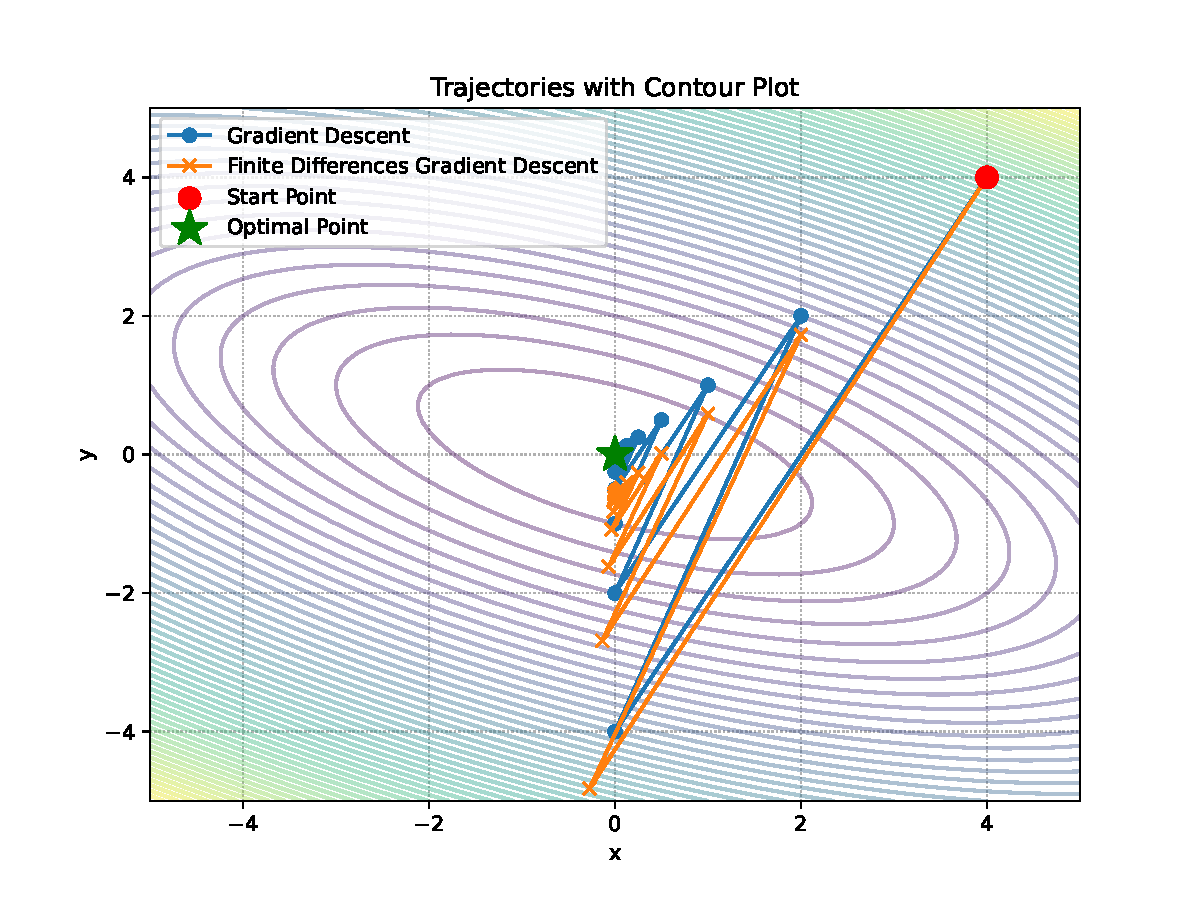
\includegraphics[keepaspectratio]{zgd_fd.pdf}}

}

\caption{``Illustration of finite differences estimator of Gradient
Descent''}

\end{figure}%
\end{column}
\end{columns}
\end{frame}

\begin{frame}{Проклятие размерности методов нулевого порядка}
\phantomsection\label{ux43fux440ux43eux43aux43bux44fux442ux438ux435-ux440ux430ux437ux43cux435ux440ux43dux43eux441ux442ux438-ux43cux435ux442ux43eux434ux43eux432-ux43dux443ux43bux435ux432ux43eux433ux43e-ux43fux43eux440ux44fux434ux43aux430}
\[
\min_{x \in \mathbb{R}^n} f(x)
\]

\pause

\[
\text{GD: } x_{k+1} = x_k - \alpha_k \nabla f(x_k) \qquad \qquad \text{Zero order GD: } x_{k+1} = x_k - \alpha_k G,
\]

where \(G\) is a 2-point or multi-point estimator of the gradient.

\pause

\begin{longtable}[]{@{}
  >{\centering\arraybackslash}p{(\linewidth - 6\tabcolsep) * \real{0.1304}}
  >{\centering\arraybackslash}p{(\linewidth - 6\tabcolsep) * \real{0.2174}}
  >{\centering\arraybackslash}p{(\linewidth - 6\tabcolsep) * \real{0.2609}}
  >{\centering\arraybackslash}p{(\linewidth - 6\tabcolsep) * \real{0.3913}}@{}}
\toprule\noalign{}
\begin{minipage}[b]{\linewidth}\centering
\end{minipage} & \begin{minipage}[b]{\linewidth}\centering
\(f(x)\) - smooth
\end{minipage} & \begin{minipage}[b]{\linewidth}\centering
\(f(x)\) - smooth and convex
\end{minipage} & \begin{minipage}[b]{\linewidth}\centering
\(f(x)\) - smooth and strongly convex
\end{minipage} \\
\midrule\noalign{}
\endhead
GD &
\(\|\nabla f(x_k)\|^2 \approx \mathcal{O} \left( \dfrac{1}{k} \right)\)
& \(f(x_k) - f^* \approx  \mathcal{O} \left( \dfrac{1}{k} \right)\) &
\(\|x_k - x^*\|^2 \approx \mathcal{O} \left( \left(1 - \dfrac{\mu}{L}\right)^k \right)\) \\
Zero order GD &
\(\|\nabla f(x_k)\|^2 \approx \mathcal{O} \left( \dfrac{n}{k} \right)\)
& \(f(x_k) - f^* \approx  \mathcal{O} \left( \dfrac{n}{k} \right)\) &
\(\|x_k - x^*\|^2 \approx \mathcal{O} \left( \left(1 - \dfrac{\mu}{n L}\right)^k \right)\) \\
\bottomrule\noalign{}
\end{longtable}
\end{frame}

\begin{frame}{Метод конечных разностей}
\phantomsection\label{ux43cux435ux442ux43eux434-ux43aux43eux43dux435ux447ux43dux44bux445-ux440ux430ux437ux43dux43eux441ux442ux435ux439}
The naive approach to get approximate values of gradients is
\textbf{Finite differences} approach. For each coordinate, one can
calculate the partial derivative approximation:

\[
\dfrac{\partial L}{\partial w_k} (w) \approx \dfrac{L(w+\varepsilon e_k) - L(w)}{\varepsilon}, \quad e_k = (0, \ldots, \underset{{\tiny k}}{1}, \ldots, 0)
\]

\pause

\begin{tcolorbox}[enhanced jigsaw, bottomrule=.15mm, title=\textcolor{quarto-callout-color}{\faInfo}\hspace{0.5em}{Question}, breakable, opacitybacktitle=0.6, colbacktitle=quarto-callout-color!10!white, left=2mm, bottomtitle=1mm, colback=white, colframe=quarto-callout-color-frame, titlerule=0mm, toptitle=1mm, arc=.35mm, rightrule=.15mm, coltitle=black, toprule=.15mm, opacityback=0, leftrule=.75mm]

If the time needed for one calculation of \(L(w)\) is \(T\), what is the
time needed for calculating \(\nabla_w L\) with this approach?

\pause

\textbf{Answer} \(2dT\), which is extremely long for the huge scale
optimization. Moreover, this exact scheme is unstable, which means that
you will have to choose between accuracy and stability.

\pause

\textbf{Theorem}

There is an algorithm to compute \(\nabla_w L\) in \(\mathcal{O}(T)\)
operations. \footnotemark{}

\end{tcolorbox}

\footnotetext{Linnainmaa S. The representation of the cumulative
rounding error of an algorithm as a Taylor expansion of the local
rounding errors. Master's Thesis (in Finnish), Univ. Helsinki, 1970.}
\end{frame}




\end{document}
